\section{Data Reduction and Analysis} \label{sec:reduction-analysis}
    \begin{itemize}
        \item Will contain the details of the data reduction routines used
        \item Will contain the software tools used for data analysis
    \end{itemize}
    
    \subsection{ASCA SIS1 observations}
    
    \subsection{Chandra ACIS observations}
    
    \subsection{XMM-Newton EPIC-pn observations}
    	The SSS \source\ was observed by all the instruments, viz. EPIC-MOS 1, EPIC-MOS 2, EPIC-pn and RGS, on-board the XMM-Newton observatory for $\sim 52$ ks on 16 December 2000. Whereas, we had retrieved data from all the instruments, we decided to use only the EPIC-pn data. The reason for this being two-fold:
    	\begin{enumerate}[i.]
    		\item The spectral region of interest is of the lowest energies detectable by EPIC, and the pn detector has a comparatively higher sensitivity than the MOS detectors at lower energies \cite{stecchini2023revisiting,mateos2009statistical}.
    		\item Currently, the high resolution grating spectra (such as those produced by the RGS) yield unacceptable fits to atmosphere models of SSS. Also, no atmosphere model has yet been able to reproduce all the details in such grating spectra \cite{ness2020complications}.
    	\end{enumerate}
    As per recommendations by the XMM-Newton SOC, the data analysis was restricted to energies above 0.2 keV\footnote{\url{https://xmmweb.esac.esa.int/docs/documents/CAL-TN-0018.pdf}}. The data reduction procedures were performed using the \textit{XMM-Newton Science Analysis System} (SAS) version 21.0.0.
    
    The Observation Data Files (ODF) were downloaded using the online archival query interface at the \textit{High Energy Astrophysics Science Archive Research Center} (HEASARC)\footnote{\url{https://heasarc.gsfc.nasa.gov/db-perl/W3Browse/w3browse.pl}}. In order to prepare the data for processing, we included the instrumental and calibration information by creating a Calibration Index File (CIF), which was up-to-date with the current calibration files (CCF)\footnote{\url{https://www.cosmos.esa.int/web/xmm-newton/current-calibration-files}}, and an extended ODF summary file. These were done by running the SAS tasks \texttt{cifbuild} and \texttt{odfingest} respectively. The ODFs were then reprocessed to generate the calibrated event files using the \texttt{epproc}, using the default parameters. The event file for EPIC-pn was filtered using the canned screening set of flags, and by setting \texttt{PATTERN==0} to select only single-pixel events in order to maximise energy calibration and resolution. The procedure described by Jethwa et al. (2015) \cite{jethwa2015pile} was used to check and find that the spectral distortion and flux loss both $<0.01\%$, which implied that the pile-up effects could be neglected.
    \begin{figure}[!htb]
        \centering
        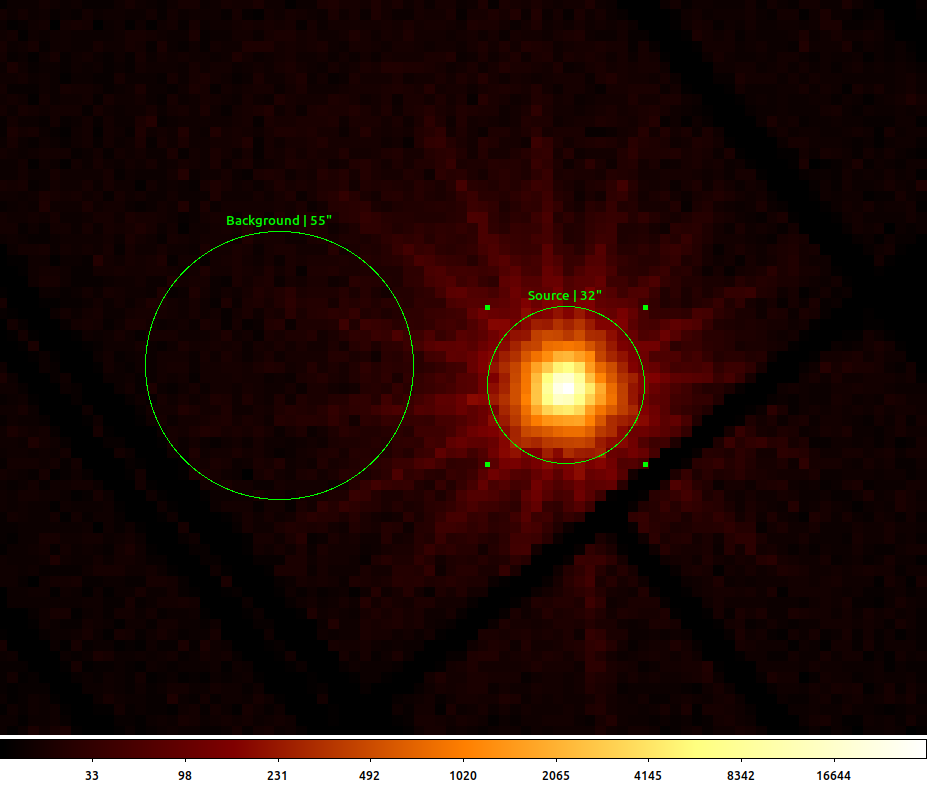
\includegraphics[width=0.45\textwidth]{figures/rx-j0925.7-4758_0111150101_src-bkg.png}
        \caption{Source and background extraction regions for the XMM-Newton observation of \source}
        \label{fig:src-bkg:pn}
    \end{figure}
    
    The source photons were extracted from a circular region having a radius of 30" which is centred at the \source\ centroid position, encompassing about 85-90\% of XMM-Newton's telescope's on-axis PSF\footnote{\url{https://xmm-tools.cosmos.esa.int/external/xmm_user_support/documentation/uhb/onaxisxraypsf.html}}. For the background photons, first the SAS task \texttt{ebkgreg} was executed to obtain an optimum circular background extraction region of radius $\sim$55". The resulting source and background extraction regions are displayed in figure \ref{fig:src-bkg:pn}. The redistribution matrix file (RMF) and ancillary response file (ARF) were generated using the standard SAS tasks \texttt{rmfgen} and \texttt{arfgen}. The spectrum was finally binned to have a minimum of 10 counts/bin using the FTOOLS task \texttt{grphha} in order to make it ready for analysis using Xspec.
    \subsection{NICER XTI observations}
    
